\documentclass{beamer}
\usepackage{pdfpages}
%Imports and customization
\usepackage{tikz}
\usepackage{graphicx}
\usepackage{tikz-feynman}
\usepackage{ulem}
\usepackage{colortbl}
\graphicspath{ 
    {./images/}
}

\beamertemplatenavigationsymbolsempty
\setbeamertemplate{sidebar right}{}
\setbeamertemplate{footline}{
    \hfill\usebeamertemplate***{navigation symbols}
    \hspace{1cm}\insertframenumber{}/\inserttotalframenumber
}
\setbeamertemplate{caption}{\raggedright\insertcaption\par}
\setbeamersize{text margin left=4mm,text margin right=4mm} 

\setbeamerfont{itemize/enumerate body}{size=\scriptsize}
\setbeamerfont{itemize/enumerate subbody}{size=\scriptsize}
\setbeamerfont{itemize/enumerate subsubbody}{size=\scriptsize}


%Custom Macros
\newcommand{\statwarn}{
    \tiny \color{red} Absolute numbers here mean NOTHING. Plots are based on small (100k events) samples, and are highly biased. All that matters is relative position!
}


% WARNING: When using these commands, the image argument must
% NOT have spaces between itself and the braces
\newcommand{\fullscreenimage}[2]{
    \frame{
        \frametitle{#1} 
        \begin{figure}
        \includegraphics[height=0.9\textheight,width=\textwidth,keepaspectratio]{#2}
        \end{figure}
    }
}


\newcommand{\importpdf}[3]{
    \frame{
        \begin{columns}\column{\dimexpr\paperwidth-10pt}
        \begin{figure}
        \includegraphics[page=#2,height=0.8\textheight,width=\textwidth,keepaspectratio]{#1}
        \end{figure}

        {\tiny #3}
        \end{columns}
    }
}


\newcommand{\displayone}[3]{
    \frame{
        \frametitle{#1} 
        \begin{columns}
            \begin{column}{0.5\textwidth}
                #2
            \end{column}
            \begin{column}{0.5\textwidth}
                \begin{figure}
                    \includegraphics[width=\linewidth,height=\textheight,keepaspectratio]{#3}
                \end{figure}
            \end{column}
        \end{columns}
    }
}

\newcommand{\displayonelarge}[3]{
    \frame{
        \frametitle{#1} 
        \begin{columns}
            \begin{column}{0.3\textwidth}
                #2
            \end{column}
            \begin{column}{0.7\textwidth}
                \begin{figure}
                    \includegraphics[width=\linewidth,height=0.8\textheight,keepaspectratio]{#3}
                \end{figure}
            \end{column}
        \end{columns}
    }
}


\newcommand{\displaytwo}[4]{
    \frame{
        \frametitle{#1} 
        #2
        \begin{columns}
            \begin{column}{0.5\textwidth}
                \begin{figure}
                    \includegraphics[width=\linewidth,height=\textheight,keepaspectratio]{#3}
                \end{figure}
            \end{column}
            \begin{column}{0.5\textwidth}
                \begin{figure}
                    \includegraphics[width=\linewidth,height=\textheight,keepaspectratio]{#4}
                \end{figure}
            \end{column}
        \end{columns}
    }
}

\newcommand{\displaytwocaption}[6]{
    \frame{
        \frametitle{#1} 
        #2
        \begin{columns}
            \begin{column}{0.5\textwidth}
                \begin{figure}
                    \includegraphics[width=\linewidth,height=\textheight,keepaspectratio]{#3}
                    \caption{#4}
                \end{figure}
            \end{column}
            \begin{column}{0.5\textwidth}
                \begin{figure}
                    \includegraphics[width=\linewidth,height=\textheight,keepaspectratio]{#5}
                    \caption{#6}
                \end{figure}
            \end{column}
        \end{columns}
    }
}

\newcommand{\displaytwoVcaption}[6]{
    \frame{
        \begin{columns}
            \begin{column}{0.5\textwidth}
                \frametitle{#1} 
                #2
            \end{column}
            \begin{column}{0.5\textwidth}
                \begin{figure}
                    \includegraphics[width=\linewidth,height=0.3\textheight,keepaspectratio]{#3}
                    \caption{#4}
                \end{figure}

                \begin{figure}
                    \includegraphics[width=\linewidth,height=0.3\textheight,keepaspectratio]{#5}
                    \caption{#6}
                \end{figure}
            \end{column}
        \end{columns}
    }
}


\newcommand{\displaythree}[5]{
    \frame{
        \begin{columns}[T]
            \begin{column}{0.4\textwidth}
                {\usebeamercolor[fg]{title} \insertframetitle{#1} }\\
                \vspace{5mm}
                #2
            \end{column}
            \begin{column}{0.4\textwidth}
                \begin{figure}
                    \includegraphics[width=\linewidth,height=\textheight,keepaspectratio]{#3}
                \end{figure}
            \end{column}
        \end{columns}
        \begin{columns}[T]
            \begin{column}{0.4\textwidth}
                \begin{figure}
                    \includegraphics[width=\linewidth,height=\textheight,keepaspectratio]{#4}
                \end{figure}
            \end{column}
            \begin{column}{0.4\textwidth}
                \begin{figure}
                    \includegraphics[width=\linewidth,height=\textheight,keepaspectratio]{#5}
                \end{figure}
            \end{column}
        \end{columns}
    }
}


\newcommand{\displayfour}[5]{
    \frame{
        \frametitle{#1} 
        \begin{columns}[T]
            \begin{column}{0.4\textwidth}
                \begin{figure}
                    \includegraphics[width=\linewidth,height=\textheight,keepaspectratio]{#2}
                \end{figure}
            \end{column}
            \begin{column}{0.4\textwidth}
                \begin{figure}
                    \includegraphics[width=\linewidth,height=\textheight,keepaspectratio]{#3}
                \end{figure}
            \end{column}
        \end{columns}
        \begin{columns}[T]
            \begin{column}{0.4\textwidth}
                \begin{figure}
                    \includegraphics[width=\linewidth,height=\textheight,keepaspectratio]{#4}
                \end{figure}
            \end{column}
            \begin{column}{0.4\textwidth}
                \begin{figure}
                    \includegraphics[width=\linewidth,height=\textheight,keepaspectratio]{#5}
                \end{figure}
            \end{column}
        \end{columns}
    }
}


\newcommand{\pstrike}[2]{
    \only<-\the\numexpr#1-1>{#2}
    \only<#1->{\sout{#2}}
}


\newcommand{\announcesection}[1]{
    \section{#1}
    \frame{
        \begin{center}
            {\huge #1} 
        \end{center}
    }
}

\newcommand{\kvv}{\kappa_{2V}}
\newcommand{\kl}{\kappa_{\lambda}}
\newcommand{\kv}{\kappa_{V}}

\newcommand{\fkvv}[1]{\kappa_{2V,#1}}
\newcommand{\fkl} [1]{\kappa_{\lambda,#1}}
\newcommand{\fkv} [1]{\kappa_{V,#1}}

\newcommand{\importpdfwpages}[3]{
    \foreach \pageN in {#2,...,#3}{
        \importpdf{#1}{\pageN}{}
    }
}

\newcommand{\hyper}[2]{{\color{blue}\href{#1}{#2}}}



%Begin Presentation
\begin{document}
    \setbeamercolor{background canvas}{bg=}
    \title{Picking a New Sample for Production}
    \author{Chris Milke}
    \date{3 June, 2021}

    \frame{\titlepage}
    \frame{\frametitle{Overview} \tableofcontents}

    \section{Introduction}
    % Show the old math intro again
    \section{Linear Algebra}

% show diagrams with terms, then show squaring
\frame{
    \frametitle{3D Coupling Dependence}
    \begin{figure}
    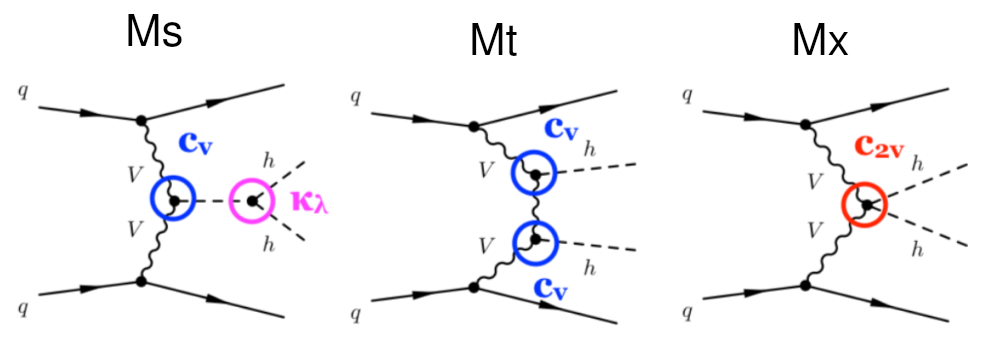
\includegraphics[width=0.6\linewidth,height=0.6\textheight,keepaspectratio]{vbf-hh_diagrams2b}
    \end{figure}
    $ \sigma = | \kv \kl M_s + \kv^2 M_t + \kvv M_x |^2 = $

    \vspace{10mm}

    $ \kv^2 \kl^2 M_s^2 + \kv^4 M_t^2 + \kvv^2 M_x^2 
    + \kv^3 \kl (M_s^* M_t + M_t^* M_s) 
    + \kv \kl \kvv (M_s^* M_x + M_x^* M_s ) 
    + \kv^2 \kvv (M_t^* M_x + M_x^* M_t )$

    \vspace{10mm}

    $ \sigma = \kv^2 \kl^2 a_1 + \kv^4 a_2 + \kvv^2 a_3 + \kv^3 \kl a_4 + \kv \kl \kvv a_5 + \kv^2 \kvv a_6 $
}

% convert to matrix, show nice matrix solution
\frame{
    \frametitle{Reweighting Solved via Linear Algebra}

    \begin{columns}[T]
        \begin{column}{0.18\textwidth}
            $ \vec{\sigma} = \begin{pmatrix} \sigma_1 \\
                \sigma_2 \\ \sigma_3 \\ \sigma_4 \\
                \sigma_5 \\ \sigma_6 \end{pmatrix} $
        \end{column}
        \begin{column}{0.15\textwidth}
            $ \vec{a} = \begin{pmatrix} a_1 \\ a_2 \\ a_3 \\ a_4 \\ a_5 \\ a_6 \end{pmatrix} $
        \end{column}
        \begin{column}{0.25\textwidth}
            $ \vec{f} = \begin{pmatrix} \kv^2 \kl^2 \\ \kv^4 \\ \kvv^2 \\ \kv^3 \kl \\ \kv \kl \kvv \\ \kv^2 \kvv \end{pmatrix} $
        \end{column}
        \begin{column}{0.4\textwidth}
            $ F = \begin{pmatrix}
                \vec{f}(\fkvv{1}, \fkl{1}, \fkv{1}) \\
                \vec{f}(\fkvv{2}, \fkl{2}, \fkv{2}) \\
                \vec{f}(\fkvv{3}, \fkl{3}, \fkv{3}) \\
                \vec{f}(\fkvv{4}, \fkl{4}, \fkv{4}) \\
                \vec{f}(\fkvv{5}, \fkl{5}, \fkv{5}) \\
                \vec{f}(\fkvv{6}, \fkl{6}, \fkv{6}) \\
            \end{pmatrix} $
        \end{column}
    \end{columns}

    \vspace{10mm}

    $ \vec{\sigma} = F \bullet \vec{a} \; \Longrightarrow \; \vec{a} = F^{-1} \bullet \vec{\sigma} $

    \vspace{10mm}

    $ \boxed{ \sigma(\kvv,\kl,\kv) = \vec{f}(\kvv,\kl,\kv) \bullet F^{-1} \bullet \vec{\sigma} } $
}

    \announcesection{$\kvv, \kl, \kv$ 3D Full Scan}

\frame{
    \frametitle{6-Term Bases}

    Over 600 Valid Combinations, 250 of which contain the SM sample.
    \vspace{5mm}

    Top 10 Bases. Samples displayed as $(\kvv, \kl, \kv)$
    \vspace{3mm}

    \resizebox{0.8\textwidth}{!}{ \begin{minipage}{1.0\textwidth}
    \begin{tabular}{ |l|l|l|l|l|l|c| }
        \hline
            \textbf {Sample 1} & \textbf {Sample 2} & \textbf {Sample 3} &
            \textbf {Sample 4} & \textbf {Sample 5} & \textbf {Sample 6} &
            \textbf {Nweight Int}\\
            \hline
            (1, 1, 1) & (0.5, 1, 1) & (3, 1, 1) & (1, 2, 1 ) & (1, 10, 1) & (0, 0, 1) &  323 \\
            (1, 1, 1) & (0.5, 1, 1) & (3, 1, 1) & (1, 0, 1 ) & (1, 10, 1) & (0, 0, 1) &  343 \\
            (1, 1, 1) & (0.5, 1, 1) & (1.5, 1, 1) & (1, 2, 1 ) & (1, 10, 1) & (0, 0, 1) &  362 \\
            (1, 1, 1) & (0.5, 1, 1) & (2, 1, 1) & (1, 2, 1 ) & (1, 10, 1) & (0, 0, 1) &  365 \\
            (1, 1, 1) & (0.5, 1, 1) & (1.5, 1, 1) & (1, 0, 1 ) & (1, 10, 1) & (0, 0, 1) &  387 \\
            (1, 1, 1) & (0, 1, 1) & (1, 2, 1) & (1, 10, 1) & (1, 1, 0.5)  & (0, 0, 1) &  390 \\
            (1, 1, 1) & (0.5, 1, 1) & (2, 1, 1) & (1, 0, 1 ) & (1, 10, 1) & (0, 0, 1) &  394 \\
            (1, 1, 1) & (0.5, 1, 1) & (1, 2, 1) & (1, 10, 1) & (1, 1, 0.5)  & (0, 0, 1) &  397 \\
            (1, 1, 1) & (0.5, 1, 1) & (1, 0, 1) & (1, 10, 1) & (1, 1, 0.5)  & (0, 0, 1) &  398 \\
            (1, 1, 1) & (0, 1, 1) & (3, 1, 1) & (1, 2, 1 ) & (1, 10, 1) & (0, 0, 1) &  400 \\
            \hline
    \end{tabular}
    \end{minipage}}
}

\frame{ \frametitle{6-Term Top Two Bases}
    Rank 1\\
    \vspace{3mm}
    \resizebox{0.8\textwidth}{!}{ \begin{minipage}{1.0\textwidth}
    {\tiny $\left(2 \kappa_{2V}^{2} - 2 \kappa_{2V} \kappa_{V}^{2} - 3 \kappa_{2V} \kappa_{V} \kappa_{\lambda} + 3 \kappa_{V}^{3} \kappa_{\lambda}\right) \times \sigma{\left(\frac{1}{2},1,1 \right)} +$

$ \left(2 \kappa_{2V}^{2} - 2 \kappa_{2V} \kappa_{V}^{2} - \kappa_{2V} \kappa_{V} \kappa_{\lambda} + \kappa_{V}^{3} \kappa_{\lambda}\right) \times \sigma{\left(\frac{3}{2},1,1 \right)} +$

$ \left(- \frac{5 \kappa_{2V} \kappa_{V}^{2}}{4} + \frac{5 \kappa_{2V} \kappa_{V} \kappa_{\lambda}}{4} + \frac{\kappa_{V}^{3} \kappa_{\lambda}}{8} - \frac{\kappa_{V}^{2} \kappa_{\lambda}^{2}}{8}\right) \times \sigma{\left(1,2,1 \right)} +$

$ \left(- \kappa_{2V} \kappa_{V}^{2} + \kappa_{2V} \kappa_{V} \kappa_{\lambda} + \kappa_{V}^{4} - \kappa_{V}^{3} \kappa_{\lambda}\right) \times \sigma{\left(0,0,1 \right)} +$

$ \left(\frac{\kappa_{2V} \kappa_{V}^{2}}{36} - \frac{\kappa_{2V} \kappa_{V} \kappa_{\lambda}}{36} - \frac{\kappa_{V}^{3} \kappa_{\lambda}}{72} + \frac{\kappa_{V}^{2} \kappa_{\lambda}^{2}}{72}\right) \times \sigma{\left(1,10,1 \right)} +$

$ \left(- 4 \kappa_{2V}^{2} + \frac{56 \kappa_{2V} \kappa_{V}^{2}}{9} + \frac{16 \kappa_{2V} \kappa_{V} \kappa_{\lambda}}{9} - \frac{28 \kappa_{V}^{3} \kappa_{\lambda}}{9} + \frac{\kappa_{V}^{2} \kappa_{\lambda}^{2}}{9}\right) \times \sigma{\left(1,1,1 \right)}$
}
    \end{minipage}}

    \vspace{7mm}

    Rank 2\\
    \vspace{3mm}
    \resizebox{0.8\textwidth}{!}{ \begin{minipage}{1.0\textwidth}
    {\tiny $\left(\frac{2 \kappa_{2V}^{2}}{3} - \frac{2 \kappa_{2V} \kappa_{V}^{2}}{3} - \frac{\kappa_{2V} \kappa_{V} \kappa_{\lambda}}{3} + \frac{\kappa_{V}^{3} \kappa_{\lambda}}{3}\right) \times \sigma{\left(2,1,1 \right)} +$

$ \left(\frac{4 \kappa_{2V}^{2}}{3} - \frac{4 \kappa_{2V} \kappa_{V}^{2}}{3} - \frac{8 \kappa_{2V} \kappa_{V} \kappa_{\lambda}}{3} + \frac{8 \kappa_{V}^{3} \kappa_{\lambda}}{3}\right) \times \sigma{\left(\frac{1}{2},1,1 \right)} +$

$ \left(- \frac{5 \kappa_{2V} \kappa_{V}^{2}}{4} + \frac{5 \kappa_{2V} \kappa_{V} \kappa_{\lambda}}{4} + \frac{\kappa_{V}^{3} \kappa_{\lambda}}{8} - \frac{\kappa_{V}^{2} \kappa_{\lambda}^{2}}{8}\right) \times \sigma{\left(1,2,1 \right)} +$

$ \left(- \kappa_{2V} \kappa_{V}^{2} + \kappa_{2V} \kappa_{V} \kappa_{\lambda} + \kappa_{V}^{4} - \kappa_{V}^{3} \kappa_{\lambda}\right) \times \sigma{\left(0,0,1 \right)} +$

$ \left(\frac{\kappa_{2V} \kappa_{V}^{2}}{36} - \frac{\kappa_{2V} \kappa_{V} \kappa_{\lambda}}{36} - \frac{\kappa_{V}^{3} \kappa_{\lambda}}{72} + \frac{\kappa_{V}^{2} \kappa_{\lambda}^{2}}{72}\right) \times \sigma{\left(1,10,1 \right)} +$

$ \left(- 2 \kappa_{2V}^{2} + \frac{38 \kappa_{2V} \kappa_{V}^{2}}{9} + \frac{7 \kappa_{2V} \kappa_{V} \kappa_{\lambda}}{9} - \frac{19 \kappa_{V}^{3} \kappa_{\lambda}}{9} + \frac{\kappa_{V}^{2} \kappa_{\lambda}^{2}}{9}\right) \times \sigma{\left(1,1,1 \right)}$
}
    \end{minipage}}
}

\displaythree{6-Term Negative Weight Heatmap}
{ \tiny
    New production (below) performs signficantly \textit{worse} than old production (right).
    \vspace{3mm}

    I think this is to do with the absence of the $\kvv,\kl,\kv = [0, 1, 0.5]$ sample, but this is unclear.
}
{old_negative_weights_toprank000}
{negative_weights_toprank0}
{negative_weights_toprank1}

\displayfour{6-Term Validation Plots}
{reco_mHH_compare_auto_top_3D_0-1_cvv0p0cl0p0cv1p0}
{reco_mHH_compare_auto_top_3D_0-1_cvv0p0cl1p0cv1p0}
{reco_mHH_compare_auto_top_3D_0-1_cvv0p5cl1p0cv1p0}
{reco_mHH_compare_auto_top_3D_0-1_cvv1p0cl0p0cv1p0}

\displayfour{6-Term More Validation Plots}
{reco_mHH_compare_auto_top_3D_0-1_cvv1p0cl10p0cv1p0}
{reco_mHH_compare_auto_top_3D_0-1_cvv1p0cl1p0cv0p5}
{reco_mHH_compare_auto_top_3D_0-1_cvv1p0cl1p0cv1p0}
{reco_mHH_compare_auto_top_3D_0-1_cvv1p0cl1p0cv1p5}

\displayfour{6-Term Even More Validation Plots}
{reco_mHH_compare_auto_top_3D_0-1_cvv1p0cl2p0cv1p0}
{reco_mHH_compare_auto_top_3D_0-1_cvv1p5cl1p0cv1p0}
{reco_mHH_compare_auto_top_3D_0-1_cvv2p0cl1p0cv1p0}
{reco_mHH_compare_auto_top_3D_0-1_cvv3p0cl1p0cv1p0}



\displayfour{6-Term Preview Plots (1/4)}
{reco_mHH_compare_preview_auto_top_3D_0-1_cvv-1p5cl-3p0cv1p0}
{reco_mHH_compare_preview_auto_top_3D_0-1_cvv-1p5cl-9p0cv1p0}
{reco_mHH_compare_preview_auto_top_3D_0-1_cvv-1p5cl14p0cv1p0}
{reco_mHH_compare_preview_auto_top_3D_0-1_cvv-1p5cl5p0cv1p0}

\displayfour{6-Term Preview Plots (2/4)}
{reco_mHH_compare_preview_auto_top_3D_0-1_cvv0p5cl-3p0cv1p0}
{reco_mHH_compare_preview_auto_top_3D_0-1_cvv0p5cl-9p0cv1p0}
{reco_mHH_compare_preview_auto_top_3D_0-1_cvv0p5cl14p0cv1p0}
{reco_mHH_compare_preview_auto_top_3D_0-1_cvv0p5cl5p0cv1p0}

\displayfour{6-Term Preview Plots (3/4)}
{reco_mHH_compare_preview_auto_top_3D_0-1_cvv2p0cl-3p0cv1p0}
{reco_mHH_compare_preview_auto_top_3D_0-1_cvv2p0cl-9p0cv1p0}
{reco_mHH_compare_preview_auto_top_3D_0-1_cvv2p0cl14p0cv1p0}
{reco_mHH_compare_preview_auto_top_3D_0-1_cvv2p0cl5p0cv1p0}

\displayfour{6-Term Preview Plots (4/4)}
{reco_mHH_compare_preview_auto_top_3D_0-1_cvv3p5cl-3p0cv1p0}
{reco_mHH_compare_preview_auto_top_3D_0-1_cvv3p5cl-9p0cv1p0}
{reco_mHH_compare_preview_auto_top_3D_0-1_cvv3p5cl14p0cv1p0}
{reco_mHH_compare_preview_auto_top_3D_0-1_cvv3p5cl5p0cv1p0}


    % Using Truth
    % Show orig Truth nWeight map
    % Show orig scatter
    % Show stat-capped Truth nWeight map
    % Show capped scatter
    \announcesection{Using Truth Samples For Prediction}

\displayfour{Post-Selection Performance (Top) VS Truth-Level (Bottom)}
{negative_weights_toprank0}
{negative_weights_toprank1}
{negative_weightsuncappedtruthRtop0}
{negative_weightsuncappedtruthRtop1}

\displayonelarge{Post-Selection/Truth-Level Correlation}{
    At first glance, truth performance appears only loosely correlated to post-selection performance.
    \vspace{4mm}

    But, performance can be made more similar by capping the statistics of the truth samples
}{Nweight_integral_VS_Nweight_uncapped_truth_integral}


\displayfour{Post-Selection Performance (Top) VS ``Capped" Truth-Level (Bottom)}
{negative_weights_toprank0}
{negative_weights_toprank1}
{negative_weightstruthRtop0}
{negative_weightstruthRtop1}


\displayonelarge{Post-Selection/Capped-Truth-Level Correlation}{
    Artificially limiting truth samples to 10\% of their events provides a much stronger correlation between truth and post-selection performance
}{Nweight_integral_VS_Nweight_truth_integral}



    % Solidarity
    % solidarity explanation from HH comb (skip reco-solidarity; maybe backup?)
    % show solidarity 2D histogram
    % cv=1 Show performance heatmap
    % show nWeight map and all three performance maps
    \announcesection{Let's Try Something Else}

\frame{
    \frametitle{Closer Look at How Combination is Done}
    {\footnotesize
        The long polynomial functions are just coefficients $c_i(\kvv,\kl,\kv)$ to the x-secs $|A_i|^2 = \sigma_i$
        The linearly combined signal distribution $\tilde{\sigma}(\kvv,\kl,\kv)$ can be viewed more simply as:

    }
    \vspace{5mm}

    $ \tilde{\sigma}(\kvv,\kl,\kv) = $
    \vspace{3mm}
    \begin{columns}
        \begin{column}{0.55\textwidth}
            \resizebox{0.8\textwidth}{!}{ \begin{minipage}{1.0\textwidth}
            {\tiny $
    \left(2 \kappa_{2V}^{2} - \frac{124 \kappa_{2V} \kappa_{V}^{2}}{9} + \frac{61 \kappa_{2V} \kappa_{V} \kappa_{\lambda}}{9} + \frac{106 \kappa_{V}^{4}}{9} - \frac{17 \kappa_{V}^{3} \kappa_{\lambda}}{3} - \frac{\kappa_{V}^{2} \kappa_{\lambda}^{2}}{9}\right) \left|{A{\left(1,1,1 \right)}}\right|^{2} +
$

$
    \left(2 \kappa_{2V}^{2} - 8 \kappa_{2V} \kappa_{V}^{2} + 3 \kappa_{2V} \kappa_{V} \kappa_{\lambda} + 6 \kappa_{V}^{4} - 3 \kappa_{V}^{3} \kappa_{\lambda}\right) \left|{A{\left(2,1,1 \right)}}\right|^{2} +
$

$
    \left(- 4 \kappa_{2V}^{2} + 20 \kappa_{2V} \kappa_{V}^{2} - 8 \kappa_{2V} \kappa_{V} \kappa_{\lambda} - 16 \kappa_{V}^{4} + 8 \kappa_{V}^{3} \kappa_{\lambda}\right) \left|{A{\left(1.5,1,1 \right)}}\right|^{2} +
$

$
    \left(16 \kappa_{2V} \kappa_{V}^{2} - 16 \kappa_{2V} \kappa_{V} \kappa_{\lambda} - 16 \kappa_{V}^{4} + 16 \kappa_{V}^{3} \kappa_{\lambda}\right) \left|{A{\left(0,1,0.5 \right)}}\right|^{2} +
$

$
    \left(\frac{4 \kappa_{2V} \kappa_{V}^{2}}{5} - \frac{4 \kappa_{2V} \kappa_{V} \kappa_{\lambda}}{5} + \frac{\kappa_{V}^{4}}{5} - \frac{3 \kappa_{V}^{3} \kappa_{\lambda}}{10} + \frac{\kappa_{V}^{2} \kappa_{\lambda}^{2}}{10}\right) \left|{A{\left(1,0,1 \right)}}\right|^{2} +
$

$
    \left(- \frac{\kappa_{2V} \kappa_{V}^{2}}{45} + \frac{\kappa_{2V} \kappa_{V} \kappa_{\lambda}}{45} + \frac{\kappa_{V}^{4}}{45} - \frac{\kappa_{V}^{3} \kappa_{\lambda}}{30} + \frac{\kappa_{V}^{2} \kappa_{\lambda}^{2}}{90}\right) \left|{A{\left(1,10,1 \right)}}\right|^{2}
$
}
            \end{minipage}}
        \end{column}
        \begin{column}{0.05\textwidth}
            \rightarrow
        \end{column}
        \begin{column}{0.4\textwidth}
            { \small
                $c_1(\kvv,\kl,\kv) \times \sigma(1,1,1   ) +$\\
                $c_2(\kvv,\kl,\kv) \times \sigma(2,1,1   ) +$\\
                $c_3(\kvv,\kl,\kv) \times \sigma(1.5,1,1 ) +$\\
                $c_4(\kvv,\kl,\kv) \times \sigma(0,1,0.5 ) +$\\
                $c_5(\kvv,\kl,\kv) \times \sigma(1,0,1   ) +$\\
                $c_6(\kvv,\kl,\kv) \times \sigma(1,10,1  )  $\\
            \par }
        \end{column}
    \end{columns}
}


\frame{
    \frametitle{Closer Look at How Combination is Done}

    $ \tilde{\sigma}(\kvv,\kl,\kv) = $

    { \small
        \hspace{20pt} $c_1(\kvv,\kl,\kv) \times \sigma(1,1,1   ) +$\\
        \hspace{20pt} $c_2(\kvv,\kl,\kv) \times \sigma(2,1,1   ) +$\\
        \hspace{20pt} $c_3(\kvv,\kl,\kv) \times \sigma(1.5,1,1 ) +$\\
        \hspace{20pt} $c_4(\kvv,\kl,\kv) \times \sigma(0,1,0.5 ) +$\\
        \hspace{20pt} $c_5(\kvv,\kl,\kv) \times \sigma(1,0,1   ) +$\\
        \hspace{20pt} $c_6(\kvv,\kl,\kv) \times \sigma(1,10,1  )  $\\
    \par }
    \vspace{5mm}

    { \footnotesize
        Neither the coefficients nor the xsecs can be looked at in isolation; they must be viewed \textit{together} as a combined product.
        \vspace{3mm}

        If the \textit{magnitude} of some $c_i\sigma_i$ products are disproportionately large for some $\kappa$ value,
        then the smaller $c_i\sigma_i$ (and their associated sample) barely contribute to the combined signal.
        \vspace{3mm}

        The combination depends on \textit{all} six samples.
        All six samples should be contributing at all points (no slackers!).
    \par }
}


\displaytwo{The Metric of Solidarity}{
    Define measure of ``closeness" of $c_i\sigma_i$ terms:
    \vspace{3mm}

    \textit{Solidarity}, $S \equiv \frac{ \sum\limits_{i=1}^6 c_i\sigma_i }{ \textrm{Stdev}(|c_i\sigma_i|) } $
    \vspace{3mm}

     {\tiny
        i.e. take the standard deviation of the \textit{absolute values} of the $c_i\sigma_i$ products,

        normalize this by their sum (the modeled x-sec at that point),

        and then take the \textit{reciprocal} of this normalized standard deviation ($S$ increases as standard deviation gets smaller).
        \par
    }


}{contribution_maxrank01}{negative_weights_toprank000}

\displayonelarge{Correlation Between Negative Weights and Solidarity}{
    Take the surface integral of the Solidarity map for every basis to produce a ``solidarity integral", and compare to Nweight Integral.
    \vspace{5mm}

    Higher Solidarity values \textit{strongly} correlate to fewer instances of negative weights
}{Nweight_integral_VS_reco_solidarity_integral}
\displayonelarge{Correlation Between Negative Weights and Theoretical Solidarity}{
    While looser, the correlation holds even when using only the VBF->HH->4b theoretical cross-section values
    \small{(NO MONTE-CARLO)}.
    \vspace{5mm}

    Can possibly be used to predict future MC productions. Further study needed.
}{Nweight_integral_VS_theory_solidarity_integral}

    \frame{
    \frametitle{Variation Scan Range}

    Wide range of values to check, brute-force approach:
    \vspace{3mm}

    \begin{itemize} {
        \item $\kvv =$ numpy.arange(-1, 4.5, 0.5)
        \item $\kl =$ numpy.arange(-9, 11, 1)
        \item $\kv =$ [ 0.5, 1, 1.5 ]
        \item 660 different variations
        \item Require all combinations to include SM and $\kl=2$ point to reduce combinatorics
        \item Each variation then has $\approx$ 227 valid possible combinations
        \item Total of $\approx$ 148,820 different combinations
    } \end{itemize}
    \vspace{3mm}

    Add each new variation to available samples one at a time,
    recalculate the solidarity integral for all possible valid combinations with the new sample in place
}

\displaytwocaption{Solidarity Histograms}{
    Each variation tested produces $\approx$ 227 combinations,
    and each combination has its own solidarity integral.
}
{projective_solidarity_all}{Overview of all 660 variations (sorted by Sum-Total of all integrals)}
{projective_solidarity_dump}{Closer look at top 10 variations}

\displaytwo{Performance Predictions}{
    Sum together the solidarity integrals of all possible combinations to produce a heatmap of potential improvement.
    \vspace{3mm}

    Improvement largely seems to come from placing a sample in the middle of the poor-performing regions
}
{negative_weights_toprank0}
{solidarity_performance_kv1}

\displaythree{Performance Predictions with Different $\kv$}{
    Variations with non-SM $\kv$ values can also potentially help
}
{solidarity_performance_kv0.5}
{solidarity_performance_kv1}
{solidarity_performance_kv1.5}



%\displayfour{Post-Selection Performance (Top) VS Truth-Level (Bottom)}
%{negative_weights_toprank0}
%{negative_weights_toprank1}
%{negative_weightsuncappedtruthRtop0}
%{negative_weightsuncappedtruthRtop1}
%
%\displayonelarge{Post-Selection/Truth-Level Correlation}{
%    At first glance, truth performance appears only loosely correlated to post-selection performance.
%    \vspace{4mm}
%
%    But, performance can be made more similar by capping the statistics of the truth samples
%}{Nweight_integral_VS_Nweight_uncapped_truth_integral}
%
%
%\displayfour{Post-Selection Performance (Top) VS ``Capped" Truth-Level (Bottom)}
%{negative_weights_toprank0}
%{negative_weights_toprank1}
%{negative_weightstruthRtop0}
%{negative_weightstruthRtop1}
%
%
%\displayonelarge{Post-Selection/Capped-Truth-Level Correlation}{
%    Artificially limiting truth samples to 10\% of their events provides a much stronger correlation between truth and post-selection performance
%}{Nweight_integral_VS_Nweight_truth_integral}
%

    
    % Final validation
    % show truth nWeight and validation plots for top picks
    \announcesection{Recommendations}

\displayfour{$\kvv=3, \kl=4, \kv=1.5$}
{errormap_dump/negative_weights_itertmp00_truth_quadrank0}
{errormap_dump/negative_weights_itertmp00_truth_quadrank1}
{errormap_dump/negative_weights_itertmp00_truth_quadrank2}
{errormap_dump/negative_weights_itertmp00_truth_quadrank3}

\displayfour{$\kvv=1, \kl=7, \kv=1.5$}
{errormap_dump/negative_weights_iterA05_truth_quadrank0}
{errormap_dump/negative_weights_iterA05_truth_quadrank1}
{errormap_dump/negative_weights_iterA05_truth_quadrank2}
{errormap_dump/negative_weights_iterA05_truth_quadrank3}

\displayfour{$\kvv=-0.5, \kl=8, \kv=0.5$}
{errormap_dump/negative_weights_iterA01_truth_quadrank0}
{errormap_dump/negative_weights_iterA01_truth_quadrank1}
{errormap_dump/negative_weights_iterA01_truth_quadrank2}
{errormap_dump/negative_weights_iterA01_truth_quadrank3}

\displayfour{$\kvv=2.5, \kl=-4, \kv=1$}
{errormap_dump/negative_weights_iterA03_truth_quadrank0}
{errormap_dump/negative_weights_iterA03_truth_quadrank1}
{errormap_dump/negative_weights_iterA03_truth_quadrank2}
{errormap_dump/negative_weights_iterA03_truth_quadrank3}

\displayfour{$\kvv=3, \kl=-6, \kv=1$}
{errormap_dump/negative_weights_iterA04_truth_quadrank0}
{errormap_dump/negative_weights_iterA04_truth_quadrank1}
{errormap_dump/negative_weights_iterA04_truth_quadrank2}
{errormap_dump/negative_weights_iterA04_truth_quadrank3}

\displayfour{$\kvv=1, \kl=-5, \kv=0.5$}
{errormap_dump/negative_weights_iterA00_truth_quadrank0}
{errormap_dump/negative_weights_iterA00_truth_quadrank1}
{errormap_dump/negative_weights_iterA00_truth_quadrank2}
{errormap_dump/negative_weights_iterA00_truth_quadrank3}

\displayfour{$\kvv=3, \kl=-9, \kv=1$}
{errormap_dump/negative_weights_iterA02_truth_quadrank0}
{errormap_dump/negative_weights_iterA02_truth_quadrank1}
{errormap_dump/negative_weights_iterA02_truth_quadrank2}
{errormap_dump/negative_weights_iterA02_truth_quadrank3}

\announcesection{Closer Look at Top Three}

\displayfour{$(\kvv=3, \kl=-6, \kv=1)$}
{validation_dump/truth_mHH_compare_auto_iterB02_truth_top_3D_0-1_cvv0p0cl1p0cv1p0}
{validation_dump/truth_mHH_compare_auto_iterB02_truth_top_3D_0-1_cvv0p0cl4p0cv1p0}
{validation_dump/truth_mHH_compare_auto_iterB02_truth_top_3D_0-1_cvv0p0cl8p0cv1p0}
{validation_dump/truth_mHH_compare_auto_iterB02_truth_top_3D_0-1_cvv-1p0cl10p0cv0p5}

\displayfour{More $(\kvv=3, \kl=-6, \kv=1)$}
{validation_dump/truth_mHH_compare_auto_iterB02_truth_top_3D_0-1_cvv1p5cl-1p0cv1p0}
{validation_dump/truth_mHH_compare_auto_iterB02_truth_top_3D_0-1_cvv2p0cl1p0cv1p0}
{validation_dump/truth_mHH_compare_auto_iterB02_truth_top_3D_0-1_cvv2p0cl-5p0cv1p0}
{validation_dump/truth_mHH_compare_auto_iterB02_truth_top_3D_0-1_cvv3p0cl-5p0cv1p0}

\displayfour{$(\kvv=1, \kl=-5, \kv=0.5)$}
{validation_dump/truth_mHH_compare_auto_iterB01_truth_top_3D_0-1_cvv0p0cl1p0cv1p0}
{validation_dump/truth_mHH_compare_auto_iterB01_truth_top_3D_0-1_cvv0p0cl4p0cv1p0}
{validation_dump/truth_mHH_compare_auto_iterB01_truth_top_3D_0-1_cvv0p0cl8p0cv1p0}
{validation_dump/truth_mHH_compare_auto_iterB01_truth_top_3D_0-1_cvv-1p0cl10p0cv0p5}

\displayfour{More $(\kvv=1, \kl=-5, \kv=0.5)$}
{validation_dump/truth_mHH_compare_auto_iterB01_truth_top_3D_0-1_cvv1p5cl-1p0cv1p0}
{validation_dump/truth_mHH_compare_auto_iterB01_truth_top_3D_0-1_cvv2p0cl1p0cv1p0}
{validation_dump/truth_mHH_compare_auto_iterB01_truth_top_3D_0-1_cvv2p0cl-5p0cv1p0}
{validation_dump/truth_mHH_compare_auto_iterB01_truth_top_3D_0-1_cvv3p0cl-5p0cv1p0}

\displayfour{$(\kvv=3, \kl=-9, \kv=1)$}
{validation_dump/truth_mHH_compare_auto_iterB00_truth_top_3D_0-1_cvv0p0cl1p0cv1p0}
{validation_dump/truth_mHH_compare_auto_iterB00_truth_top_3D_0-1_cvv0p0cl4p0cv1p0}
{validation_dump/truth_mHH_compare_auto_iterB00_truth_top_3D_0-1_cvv0p0cl8p0cv1p0}
{validation_dump/truth_mHH_compare_auto_iterB00_truth_top_3D_0-1_cvv-1p0cl10p0cv0p5}

\displayfour{More $(\kvv=3, \kl=-9, \kv=1)$}
{validation_dump/truth_mHH_compare_auto_iterB00_truth_top_3D_0-1_cvv1p5cl-1p0cv1p0}
{validation_dump/truth_mHH_compare_auto_iterB00_truth_top_3D_0-1_cvv2p0cl1p0cv1p0}
{validation_dump/truth_mHH_compare_auto_iterB00_truth_top_3D_0-1_cvv2p0cl-5p0cv1p0}
{validation_dump/truth_mHH_compare_auto_iterB00_truth_top_3D_0-1_cvv3p0cl-5p0cv1p0}




    %Conclusion 
    \section{Conclusion}
    \displaythree{Conclusion}{
        Highest performing samples:
        \vspace{3mm}

        \begin{itemize}
            \item $(\kvv=3, \kl=-6, \kv=1)$
            \item $(\kvv=1, \kl=-5, \kv=0.5)$
            \item $(\kvv=3, \kl=-9, \kv=1)$
        \end{itemize}
        \vspace{3mm}

        All appear to perform very well.
    }
    {errormap_dump/negative_weights_iterA04_truth_quadrank3}
    {errormap_dump/negative_weights_iterA00_truth_quadrank0}
    {errormap_dump/negative_weights_iterA02_truth_quadrank0}

    %\announcesection{Backup}

\end{document}
